\documentclass[12pt]{article}
\usepackage{amsmath}
\usepackage{array}
% \usepackage{gensymb}
\usepackage{geometry}
\usepackage{graphicx}
\usepackage{pgfplots}
\usepackage{siunitx}
\usepackage{wrapfig}

\title{Homework \#16}
\author{Donald Aingworth IV}
\date{December 11, 2024}

\pgfplotsset{width=8cm,compat=1.9}
\usepgfplotslibrary{external}
% \tikzexternalize

\begin{document}

\DeclareSIUnit{\mile}{mi}
\DeclareSIUnit{\gal}{gal}
\DeclareSIUnit{\foot}{ft}
\DeclareSIUnit{\hour}{h}
\DeclareSIUnit{\rad}{rad}
\DeclareSIUnit{\unit}{u}
\DeclareSIUnit{\dyne}{dyn}

\maketitle

\pagebreak
\section*{Question 2}
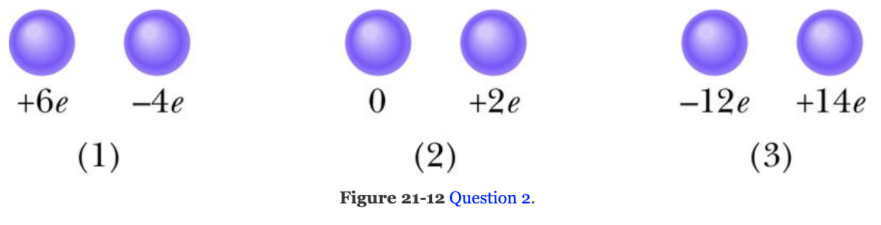
\includegraphics[width=\textwidth]{picture_1.png}
Figure 21-12 shows three pairs of identical spheres that are to be touched together and then separated. The initial charges on them are indicated. Rank the pairs according to (a) the magnitude of the charge transferred during touching and (b) the charge left on the positively charged sphere, greatest first.

\subsection*{Solution}
a) (3) $>$ (1) $>$ (2)\\
In this problem, we just need to rank the differences between the charges on the balls. In instance 1, the difference is $6 - (-4) = 10$. In instance 2, the difference is $2 - 0 = 2$. In instance 3, the difference is $14 - (-12) = 26$. We can then rank the three, and the result is \boxed{(3) > (1) > (2)}.\\
b) (1) = (2) = (3)
In this In this problem, we just need to rank the average charge of each of the two balls. In instance 1, the average is $\frac{6 + (-4)}{2} = 1$. In instance 2, the difference is $\frac{2 + 0}{2} = 1$. In instance 3, the difference is $\frac{14 + (-12)}{2} = 1$. We can then rank the three, and the result is \boxed{(1) = (2) = (3)}.


\pagebreak
\section*{Question 8}
% \begin{wrapfigure}{r}{0.15\textwidth}
%     \vspace{-30pt}
    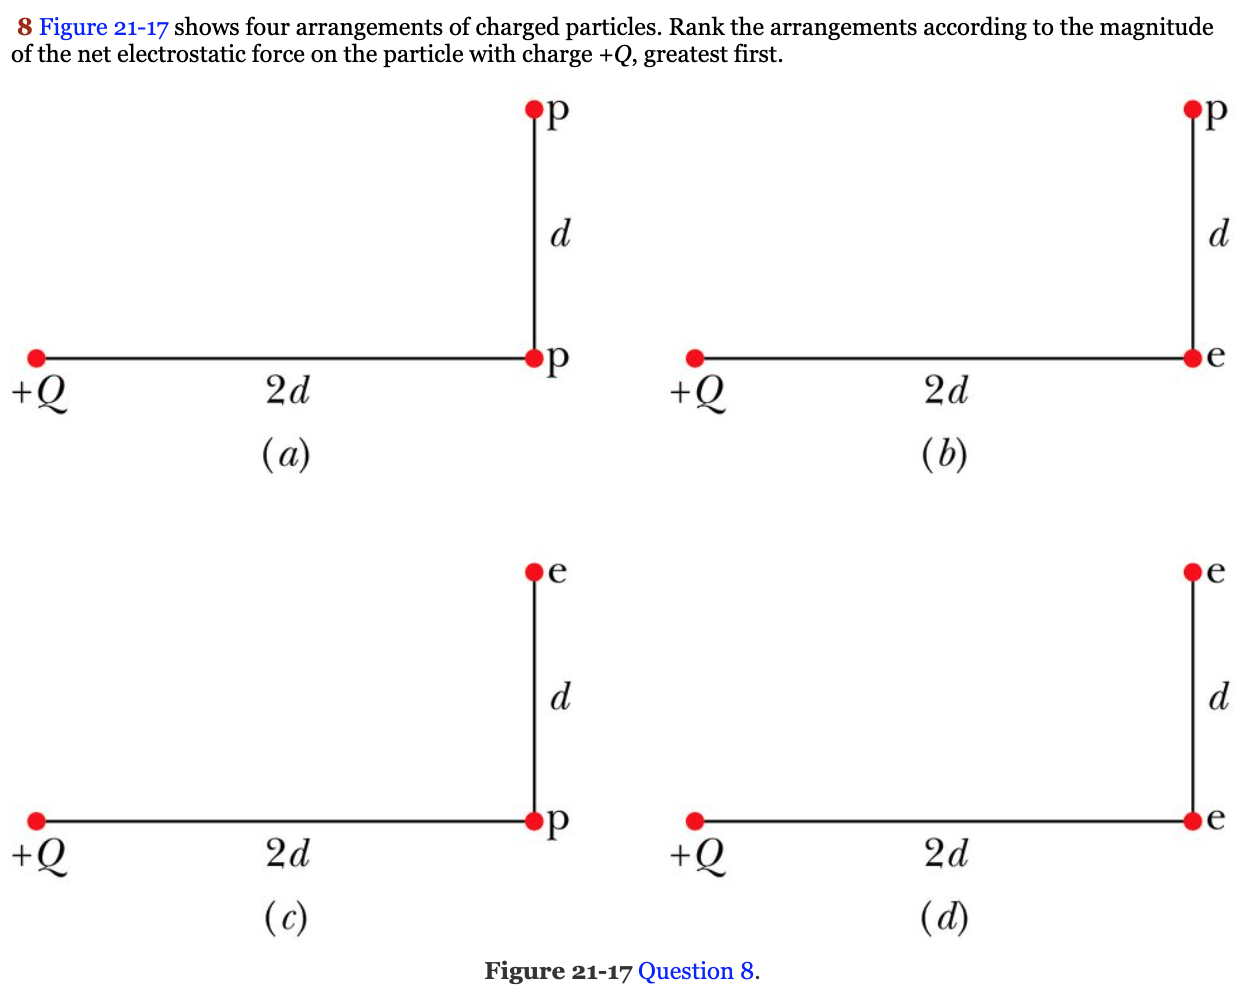
\includegraphics[width=\textwidth]{picture_2.png} 
%     % \label{fig:wrapfig}
% \end{wrapfigure}

\subsection*{Solution}
\subsubsection*{(a) = (d) $>$ (b) = (c)}
For (a) and (d), the magnitude is always positive and the charge of a positron is the same as the charge of an electron, and the other particles are working together to move +Q more than separately. This means that they have the same magnitude.\\
For (b) and (c), the magnitude is always positive, but the two charged particles are exerting force on the +Q particle in relatively opposite directions. This means that the net force on the +Q particle is the same, but it is less than the net force on it in (a) or (d).\\
Hence, \boxed{(a) = (d) > (b) = (c)}


\pagebreak
\section*{Question 10}
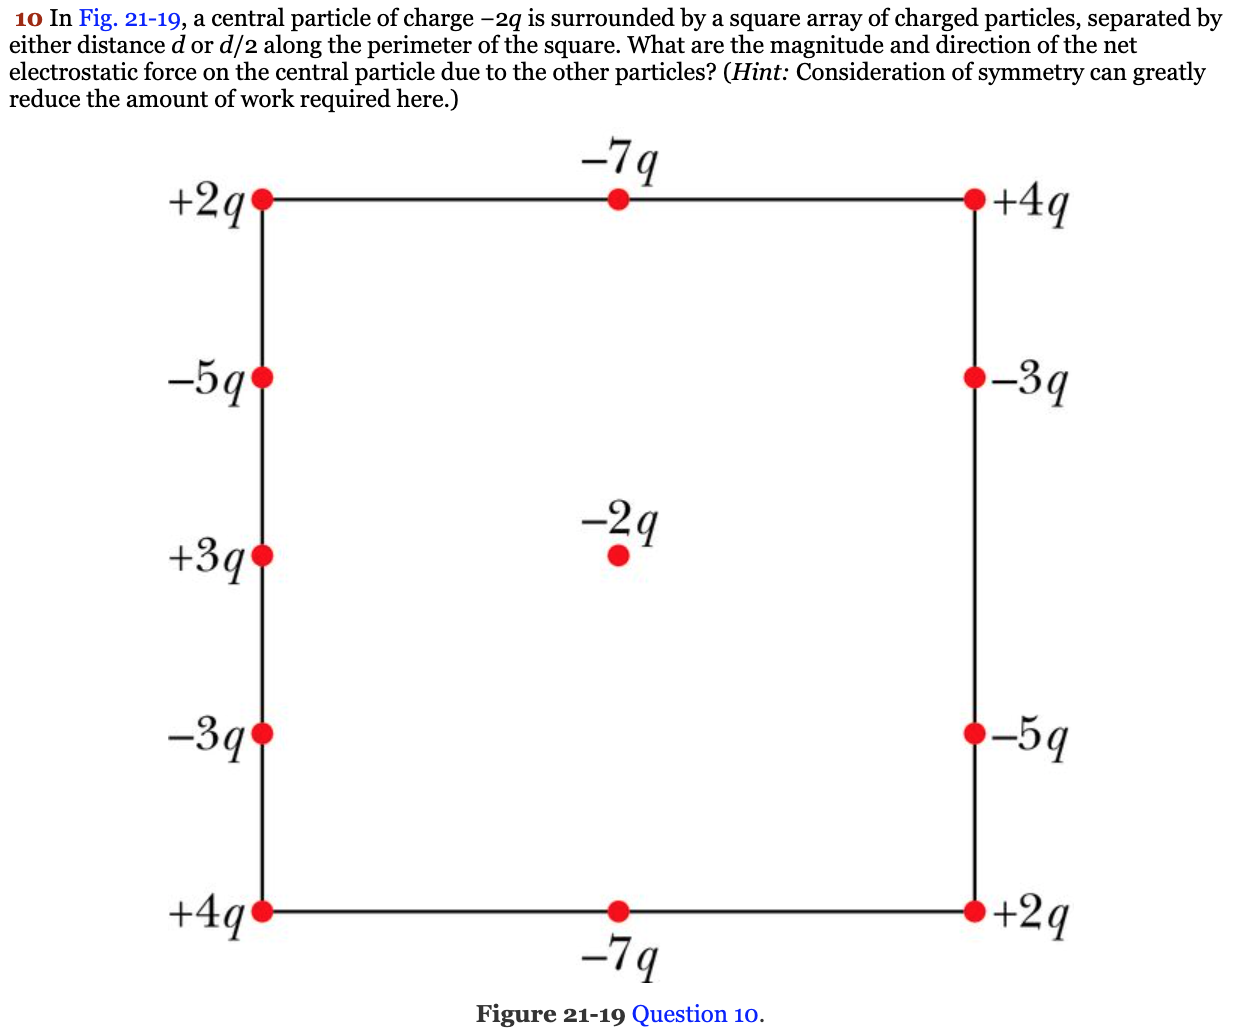
\includegraphics[width=\textwidth]{picture_3.png} 

\subsection*{Solution}
In this case, the first thing we can do is rule out the charges with charges of equal magnitude and equal distance to the central charge. Almost all charges are canceled out, as follows (in clockwise order): \(-7q; +4q; -3q; -5q; +2q\). The only remaining charge is $+3q$. As such, we can find the net force using only the force from that remaining charge. Since the charges of $+3q$ and $-2q$ are opposite and opposites attract, the direction is towards the $+3q$ charge, so to the \boxed{left}.
\[F = \frac{k\left|q_1\right|\left|q_2\right|}{r^2} 
    = \frac{k\left|3q\right|\left|-2q\right|}{d^2} 
    = \boxed{\frac{6kq^2}{d^2}} \]

\pagebreak
\section*{Problem 10}
\begin{wrapfigure}{r}{0.25\textwidth}
    \vspace{-50pt}
    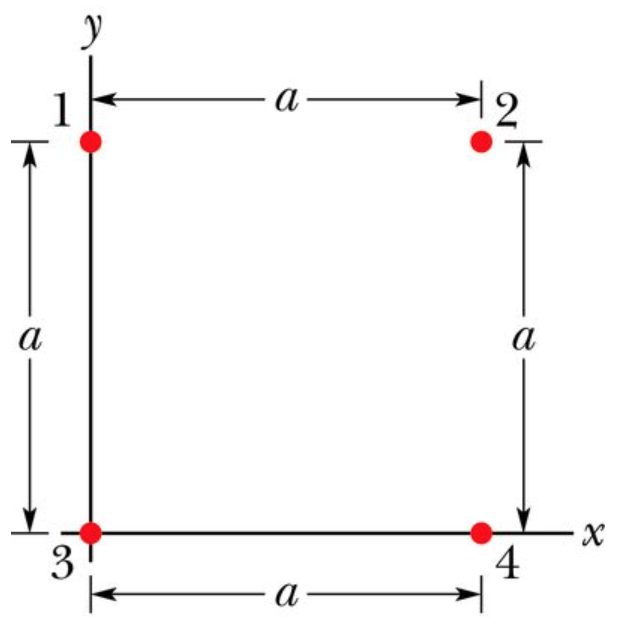
\includegraphics[width=0.25\textwidth,height=0.25\textwidth]{picture_4.png} 
    % \label{fig:wrapfig}
\end{wrapfigure}
In Fig. 21-25, four particles form a square. The charges are $q_1 = q_4 = Q$ and $q_2 = q_3 = q$. (a) What is Q/q if the net electrostatic force on particles 1 and 4 is zero? (b) Is there any value of $q$ that makes the net electrostatic force on each of the four particles zero? Explain.

\subsection*{Solution}
The distance between particles 1 \& 4 (and 2 \& 3) is found by the pythagorean theorem.
\[r_{14} = r_{23} = \sqrt{a^2 + a^2} = a\sqrt{2}\]

\subsubsection*{(a) Find Q/q}
From this, we know that net electrostatic force on 1 from 4 in the direction of the line between 1 and 2 has to be equal to the force on 1 from 4. Roughly the same applies in the direction of the line between 1 and 3. As such, we can write a formula for the net force (which is 0).
\begin{align*}
    F_{net} = 0 = \frac{k\left|q_1\right|\left|q_2\right|}{r^2} &- \frac{k\left|q_1\right|\left|q_4\right|}{r^2}*\cos(\theta)\\
    \frac{k\left|q_1\right|\left|q_2\right|}{r^2} &= \frac{k\left|q_1\right|\left|q_4\right|}{r^2}*\cos(\theta)\\
    \frac{k\left|Q\right|\left|q\right|}{a^2} &= \frac{k\left|Q\right|\left|Q\right|}{(a\sqrt{2})^2}*\cos(\theta)\\
    \frac{\left|q\right|}{a^2} &= \frac{\left|Q\right|}{2a^2}*\frac{\sqrt{2}}{2}\\
    \frac{\left|Q\right|}{\left|q\right|} = \left|\frac{Q}{q}\right| &= \frac{4}{\sqrt{2}} = 2\sqrt{2}
\end{align*}
Since the forces must be in opposite directions, the charges must be opposite, so the ration has to be negative. This means that \boxed{Q/q = -2\sqrt{2}}.

\pagebreak
\subsubsection*{(b) For what $q$ is $F_{net} = 0$?}
We can put aside the situation where \boxed{q = 0}, since that feels like cheating. We have two formulas that must be true, one for the particles of charge $Q$ (1) and one for the particles of charge $q$ (2). 
\begin{equation}
    0 = \frac{k*|q|*|Q|}{a^2} - \frac{k*|q|*|q|}{(a\sqrt{2})^2}
\end{equation}
\begin{equation}
    0 = \frac{k*|q|*|Q|}{a^2} - \frac{k*|Q|*|Q|}{(a\sqrt{2})^2}
\end{equation}

Adding these two together, we get:
\begin{equation}
    0 = \frac{k*|Q|*|Q|}{(a\sqrt{2})^2} - \frac{k*|q|*|q|}{(a\sqrt{2})^2}
\end{equation}

We can then substitute in a prior value of Q. $Q/q = -2\sqrt{2} \rightarrow Q = -2\sqrt{2}q$. 
\begin{equation}
    0 = \frac{k*Q^2 - k*q^2}{2a^2} = \frac{k(8q^2 - q^2)}{2a^2} = \frac{7kq^2}{2a^2}
\end{equation}

Since $\frac{7k}{2a^2}$ is made up only of constants, this means that we end up with $q^2 = 0$, so there is \boxed{\text{no other solution besides } q = 0}.


\pagebreak
\section*{Problem 11}
\begin{wrapfigure}{r}{0.25\textwidth}
    \vspace{-30pt}
    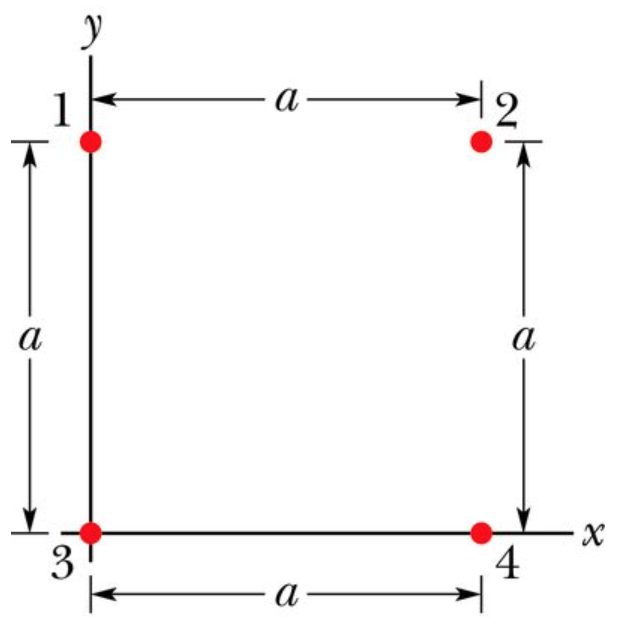
\includegraphics[width=0.25\textwidth]{picture_4.png} 
    % \label{fig:wrapfig}
\end{wrapfigure}
In Fig. 21-25, the particles have charges $q_1 = -q_2 = 100 \unit{\nano\coulomb}$ and $q_3 = -q_4 = 200 \unit{\nano\coulomb}$, and distance $a = 5.0\unit{\centi\meter}$. What are the (a) x and (b) y components of the net electrostatic force on particle 3?

\subsection*{Solution}
\subsubsection*{(a) x-force on particle 3}
From the previous problem, we have determined the formula for the x-value of the force.
\begin{align*}
    F_{net} &=  \frac{k*|q_3||q_4|}{a^2} + \frac{k*|q_3||q_2|}{2a^2}*\hat{r}_{23;x}
            =   \frac{k*|q_3||q_4|}{a^2} + \frac{k*|q_3||q_2|}{2a^2}*\hat{r}_{23;x}
\end{align*}



% \pagebreak
% \section*{Problem 23}
% \begin{wrapfigure}{r}{0.25\textwidth}
%     \vspace{-30pt}
%     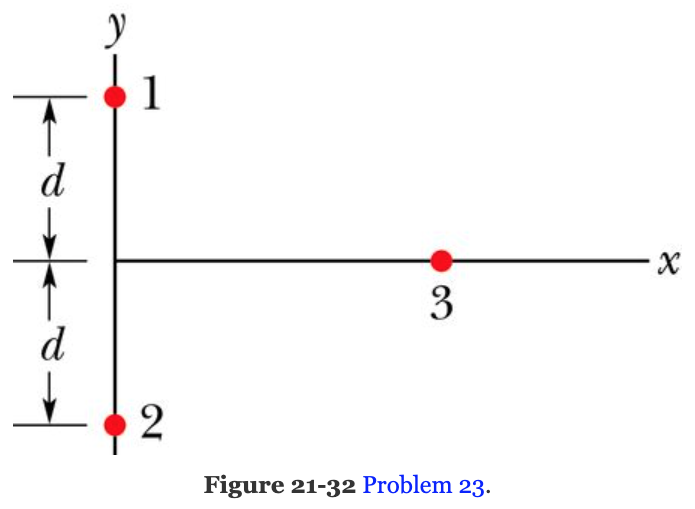
\includegraphics[width=0.25\textwidth]{picture_6.png} 
%     % \label{fig:wrapfig}
% \end{wrapfigure}
% Fig. 21-32, particles 1 and 2 of charge 91 = Q2 = +3.20 × 10-19 C are on a y axis at distance d = 17.0 cm from the origin. Particle 3 of charge 93 = +6.40 × 10-19 C is moved gradually along the x axis from x = O to x = +5.0 m. At what values of x will the magnitude of the electrostatic force on the third particle from the other two particles be (a) minimum and (b) maximum? What are the (c) minimum and (d) maximum magnitudes?

% \pagebreak
% \section*{Problem 31}
% 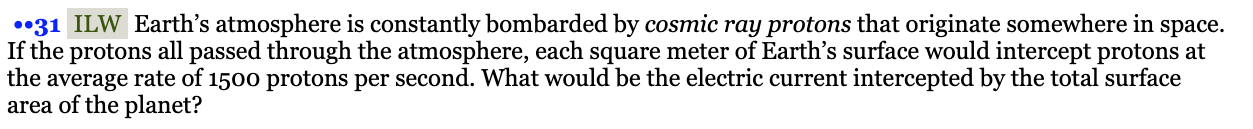
\includegraphics[width=\textwidth]{picture_7.png} 

% \pagebreak
% \section*{Problem 36}
% 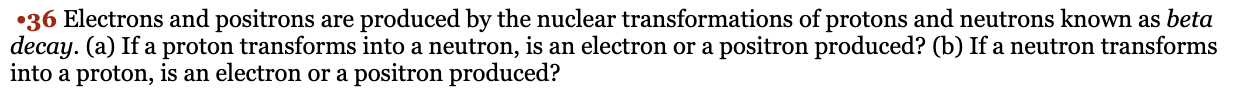
\includegraphics[width=\textwidth]{picture_8.png} 


\end{document}